% Section 8. Sources: 1201_upper_structures/FINAL.md (plateau, binding rows, edge-class inventory, structural variants,
% extrapolation DA5, run progress); 1203_ceiling_ladder/FINAL.md section 0 (ceilings Lambda_K, family rank, full model
% at r = 10); 1228_combined_lower/FINAL.md sections 6, 8 and row EB4 (diminishing increments); ledger/STATE.md rows
% mu upper and mu lower; HANDOVER_2026-10-12_wave_1200.md sections 2-3 and addendum section 4 (exact radius-7
% coordinates, levers); 809_flow_certificate_scaling/FINAL.md section 1 (1.3/r^3) and section 2 (certificates by radius);
% 1007/1201 (paired certificates r4, r6, r8, r9); web TapeMachineWriteup.tsx (single-weight tape certificates r10-r12).
%%%%%%%%%%%%%%%%%%%%%%%%%%%%%%%%%%%%%%%%%%%%%%%%%%%%%%%%%%%%%%%%%%%%%%%%
\section{Limits of the methods}\label{sec:limits}
%%%%%%%%%%%%%%%%%%%%%%%%%%%%%%%%%%%%%%%%%%%%%%%%%%%%%%%%%%%%%%%%%%%%%%%%

Figure~\ref{fig:radius} shows the certified bounds of both methods against the radius. Both improve steadily and
slowly, and extrapolation suggests that neither reaches the estimate $12.2629$ at a radius that can be computed with
the present families of weights and flows. Apart from the certified values in the figure, the statements in this
section are numerical observations and extrapolations, not theorems.

\begin{figure}[htb]
\centering
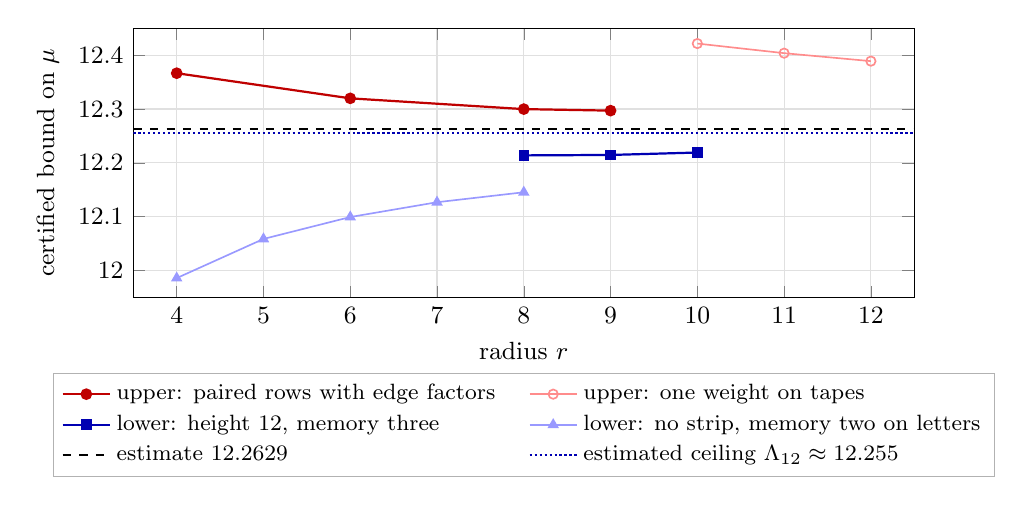
\begin{tikzpicture}
\begin{axis}[width=11.5cm,height=5.0cm,xlabel={radius $r$},ylabel={certified bound on $\mu$},
  xmin=3.5,xmax=12.5,ymin=11.95,ymax=12.45,grid=major,grid style={black!12},
  ytick={12.0,12.1,12.2,12.3,12.4},yticklabel style={/pgf/number format/fixed,/pgf/number format/precision=1},
  legend style={at={(0.5,-0.28)},anchor=north,font=\footnotesize,draw=black!30,legend columns=2,
    /tikz/every even column/.append style={column sep=1em}},legend cell align=left,
  tick label style={font=\small},label style={font=\small}]
\addplot[mark=*,mark size=1.7pt,line width=0.8pt,red!75!black] coordinates
  {(4,12.366448572318)(6,12.319749766858)(8,12.299756359)(9,12.296933854)};
\addlegendentry{upper: paired rows with edge factors}
\addplot[mark=o,mark size=1.7pt,line width=0.6pt,red!45!white] coordinates
  {(10,12.421514463859)(11,12.403654977316)(12,12.388844617135)};
\addlegendentry{upper: one weight on tapes}
\addplot[mark=square*,mark size=1.5pt,line width=0.8pt,blue!70!black] coordinates
  {(8,12.213777757442)(9,12.214596070132)(10,12.219100857094)};
\addlegendentry{lower: height 12, memory three}
\addplot[mark=triangle*,mark size=1.8pt,line width=0.6pt,blue!40!white] coordinates
  {(4,11.985857574)(5,12.058577430)(6,12.099279121)(7,12.126797697)(8,12.145297924)};
\addlegendentry{lower: no strip, memory two on letters}
\addplot[dashed,line width=0.7pt,black] coordinates {(3.5,12.262874)(12.5,12.262874)};
\addlegendentry{estimate $12.2629$}
\addplot[densely dotted,line width=0.8pt,blue!70!black] coordinates {(3.5,12.255)(12.5,12.255)};
\addlegendentry{estimated ceiling $\Lambda_{12}\approx12.255$}
\end{axis}
\end{tikzpicture}
\caption{Certified bounds by radius: paired upper certificates, earlier single-weight upper certificates, the stages
of Table~\ref{tab:lower} (last stage only at radius $10$), and earlier flows without a strip. The dotted line is an
extrapolated estimate of $\Lambda_{12}$, which caps every lower bound on the strip of height $12$.}
\label{fig:radius}
\end{figure}

\subsection{The upper bound}

\emph{Many rows are nearly tight.} The optimized certificate is a plateau: a large share of the formal rows have row
values close to the maximum. At the radius-$8$ certificate, $45$ percent of the groups of formal rows related by
reflection lie within $10^{-4}$ of the largest row value, and $53$ percent after a longer optimization; only $218$
groups lie within $10^{-5}$. So the bound is not held up by a few bad rows that a local repair could fix. The nearly
tight rows are the typical ones: the numbers of $+$ and $-$ in the row differ by $1$ or $3$, the signs change often,
and the run of equal letters at the head is short. Rows with a large imbalance or long runs have slack above $0.01$,
that is, their row values are at least $0.01$ below the maximum.

\emph{No unused freedom in the family.} Every kind of edge already carries a factor, and each part of the weight
already reads as far as the formal row allows, so within the family only a longer row helps. Adding weight factors
that count letters or sign changes beyond the row changes the bound by less than $10^{-5}$. Adaptive refinement of the
tables gets $82$ percent of the gain of the next radius from half of its new table entries, but does not reduce the
number of formal rows to check.

\emph{Cost and projection.} The number of formal rows grows fourfold per unit of radius. The radius-$9$ run was stopped
before it converged, still gaining about $10^{-4}$ per ten minutes. Extrapolating the converged optima at radius $4$,
$5$, $6$ and $8$ suggests about $12.2935$ for the radius-$9$ family and $12.289$ at radius $10$: less than $0.01$ per
step, at four times the cost. This is an extrapolation, not a bound.

\subsection{The lower bound}

\emph{The strip caps the bound.} Every flow on the strip of height $12$ gives at most $\Lambda_{12}$, the growth rate
of meanders whose labels stay in $-6\le g\le6$. Extrapolation from heights $2$ to $8$ puts $\Lambda_{12}$
near $12.255$ (plausible range $12.245$ to $12.261$), $\Lambda_{10}$ near $12.239$ and $\Lambda_{14}$ near $12.260$.
The cap does not limit the present bound, but it will once the radius and the family improve enough.

\emph{The radius and the family.} The best bound from any flow at radius $10$ and height $12$, not only from flows
of the form used here, is estimated at $12.22$ to $12.24$. At small size the four-move cycles span only $54$ to $57$ percent of the stationary directions; walks of six
and eight moves recover part of the rest. The last two increments of $131{,}072$ directions gained $0.00186$ and
$0.00076$.
% UNVERIFIED: "about 0.0003" for a third increment is a one-ratio guess in 1228; not quoted.
The next steps, in the order the computations suggest, are more complete stationary directions with a joint
optimization of all coefficients, a reference law optimized at the radius of the certificate, and then height $14$.
An exact parent at radius $7$ could not be computed within $3$~GB of memory and $45$ minutes.

\subsection{Summary}

Both methods see a bounded neighborhood of the head, and both gaps to the estimate close only as fast as that
neighborhood grows. We found nothing that changes this rate. Proving $12.26\le\mu\le12.27$ would need the lower bound to gain about $0.041$,
beyond the estimated cap of height $12$, and the upper bound about $0.027$.
